\scanpage{28}
% archive sheet number: 27

\[
\varphi(a_j,a_{\unsure{l|k|i}})=0\quad -1\leq j<l\leq n,\ l\ne j+1,\quad
\varphi(a_{-1},a_{-1})=f(a_{-1})=0
\]

\[
\begin{aligned}
0\leq i\leq n\qquad &c_i=f(a_i)=\varphi(a_i,a_i)\\
0\leq i\leq n\qquad &\lambda_i-1=\langle a_i,a'_i\rangle\\
0\leq i\leq n-1\qquad &\beta_i=\langle a_{i+1},a'_i\rangle\\
-1\leq i\leq n-1\qquad &\langle a_i,a'_{i+1}\rangle=1
\end{aligned}
\]

\[
\boxed{\begin{aligned}
&\left\{c_i\langle a_j,a'_i\rangle\deleted{\unsure{+|=|-}}\inserted{=}\overbrace{(\lambda_i-1)}^{\mu_i}\varphi(a_j,a_i)=0\right.\\
&0\leq i,\deleted{\unsure{j}}{}\leq n\qquad\lambda_i\overline{\lambda_i}=1\\
&-1\leq j\leq n
\end{aligned}}
\]
\[
\left[f(a)a'=\underbrace{\langle a,a'\rangle}_{\mu=\lambda-1}\psi(a)\right]
\]
\[
\tau x=x+\left(\frac{\mu}{f(a)}\varphi(x,a)\right)a,\qquad \lambda\bar\lambda=1
\]

\[
d_i=\frac{c_i}{\lambda_i-1}=\varphi(a_{i-1},a_i)\quad
0\leq i\leq n\qquad\text{i.e.}\quad c_i=(\lambda_i-1)d_i=\mu_i d_i
\]
\[
d_{i+1}=\overline{\beta_i}\,\overline{d_i}\qquad\text{donc}
\]
\[
\begin{aligned}
d_1&=\overline{\beta_0}\,\overline{d_0}\\
d_2&=\overline{\beta_1}\,\beta_0 d_0\\
d_3&=\overline{\beta_2}\,\beta_1\overline{\beta_0}d_0\\
&\cdots\\
d_{\deleted{\unsure{2i-1}}2i}&=\overline{\beta_{2i-1}}\beta_{2i-2}\overline{\beta_{2i-3}}\cdots\beta_0d_0\\
d_{2i+1}&=\overline{\beta_{2i}}\beta_{2i-1}\overline{\beta_{2i-2}}\cdots\overline{\beta_0}\,\overline{d_0}\\
&\cdots\\
d_{\unsure{n|n+1}}&=\overline{\beta_{n-1}}\beta_{n-2}\overline{\beta_{n-3}}\cdots
\left\}\begin{array}{ll}\beta_0d_0&\text{si }n\text{ pair}\\\overline{\beta_0}d_0&\text{si }n\text{ impair}\end{array}\right.
\end{aligned}
\]
\[
d_0=\frac{c_0}{\lambda_0-1}=\frac{c_0}{\mu_0}\ \Big|\ \underline{c_0\in k_0}
\qquad \text{OPS }c_0=1,\ \text{donc }d_0=\frac{1}{\mu_0}
\]

\[
\begin{aligned}
f(a_{-1})&=0\\
f(a_0)&=1\\
f(a_1)&=\frac{\mu_1\deleted{\unsure{1}}}{\overline{\mu_0}\deleted{\unsure{1}}}\overline{\beta_0}\\
f(a_2)&=\frac{\mu_2\deleted{\unsure{-1}}}{\mu_0^{\deleted{\unsure{\overline{\phantom{a}}}}}\deleted{\unsure{-1}}}\overline{\beta_1}\beta_0\\
f(a_3)&=\frac{\mu_3}{\overline{\mu_0}}\overline{\beta_2}\beta_1\overline{\beta_0}\\
&\cdots
\end{aligned}
\]

Supposons les $\beta_i\in k_0$, il reste les conditions
\[
\begin{aligned}
\mu_i/\mu_0^{\deleted{\unsure{\bar{\phantom{a}}}}}&\in k_0\quad\text{si }\unsure{0|i}\text{ pair}\\
\mu_{\unsure{i|1}}/\overline{\mu_0}&\in k_0\quad\text{si }i\text{ impair}
\end{aligned}
\]

\[
\begin{aligned}
\deleted{\unsure{\text{Si }\lambda}}\quad\lambda_i-1&=\rho_i(\lambda_0-1)
\quad \inserted{\text{($\rho_i\in k_0$)}}\quad i\text{ pair}\\
\lambda_i&=\rho_i(\lambda_0-1)+1\qquad\unsure{\rho}\\
\deleted{\unsure{\lambda_i\overline{\lambda_i}}}&=(\lambda_0-1)\unsure{\bar\rho_i|\bar\varphi_i|\varrho_i|q_i}
\end{aligned}
\]

\deleted{\unsure{Or}} \deleted{\unsure{Supp.}}

\[
(\lambda_1-1)=\deleted{\unsure{\rho}}c(\overline{\lambda_0}-1)
\]

\figure{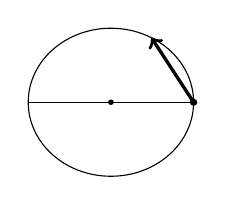
\begin{tikzpicture}[x=1.05cm,y=1cm]
\draw (0,0) ellipse (1 and .94);
\draw (-1,0) -- (1,0);
\fill (0,0) circle (.035);
\fill (1,0) circle (.045);
\draw[very thick,->] (1,0) -- (.49,.82);
\end{tikzpicture}}
